\newcommand{\svcourse}{CST Part IA: Software Engineering and Security}
\newcommand{\svnumber}{1}
\newcommand{\svvenue}{Microsoft Teams}
\newcommand{\svdate}{2022-05-11}
\newcommand{\svtime}{15:00}
\newcommand{\svuploadkey}{CBd13xmL7PC1zqhNIoLdTiYUBnxZhzRAtJxv/ytRdM1r7qIfwMsxeVwM/pPcIo8l}

\newcommand{\svrname}{Dr Sam Ainsworth}
\newcommand{\jkfside}{oneside}
\newcommand{\jkfhanded}{yes}

\newcommand{\studentname}{Harry Langford}
\newcommand{\studentemail}{hjel2@cam.ac.uk}


\documentclass[10pt,\jkfside,a4paper]{article}

% DO NOT add \usepackage commands here.  Place any custom commands
% into your SV work files.  Anything in the template directory is
% likely to be overwritten!

\usepackage{fancyhdr}

\usepackage{lastpage}       % ``n of m'' page numbering
\usepackage{lscape}         % Makes landscape easier

\usepackage{verbatim}       % Verbatim blocks
\usepackage{listings}       % Source code listings
\usepackage{graphicx}
\usepackage{float}
\usepackage{epsfig}         % Embed encapsulated postscript
\usepackage{array}          % Array environment
\usepackage{qrcode}         % QR codes
\usepackage{enumitem}       % Required by Tom Johnson's exam question header

\usepackage{hhline}         % Horizontal lines in tables
\usepackage{siunitx}        % Correct spacing of units
\usepackage{amsmath}        % American Mathematical Society
\usepackage{amssymb}        % Maths symbols
\usepackage{amsthm}         % Theorems

\usepackage{ifthen}         % Conditional processing in tex

\usepackage[top=3cm,
            bottom=3cm,
            inner=2cm,
            outer=5cm]{geometry}

% PDF metadata + URL formatting
\usepackage[
            pdfauthor={\studentname},
            pdftitle={\svcourse, SV \svnumber},
            pdfsubject={},
            pdfkeywords={9d2547b00aba40b58fa0378774f72ee6},
            pdfproducer={},
            pdfcreator={},
            hidelinks]{hyperref}

\renewcommand{\headrulewidth}{0.4pt}
\renewcommand{\footrulewidth}{0.4pt}
\fancyheadoffset[LO,LE,RO,RE]{0pt}
\fancyfootoffset[LO,LE,RO,RE]{0pt}
\pagestyle{fancy}
\fancyhead{}
\fancyhead[LO,RE]{{\bfseries \studentname}\\\studentemail}
\fancyhead[RO,LE]{{\bfseries \svcourse, SV~\svnumber}\\\svdate\ \svtime, \svvenue}
\fancyfoot{}
\fancyfoot[LO,RE]{For: \svrname}
\fancyfoot[RO,LE]{\today\hspace{1cm}\thepage\ / \pageref{LastPage}}
\fancyfoot[C]{\qrcode[height=0.8cm]{\svuploadkey}}
\setlength{\headheight}{22.55pt}


\ifthenelse{\equal{\jkfside}{oneside}}{

 \ifthenelse{\equal{\jkfhanded}{left}}{
  % 1. Left-handed marker, one-sided printing or e-marking, use oneside and...
  \evensidemargin=\oddsidemargin
  \oddsidemargin=73pt
  \setlength{\marginparwidth}{111pt}
  \setlength{\marginparsep}{-\marginparsep}
  \addtolength{\marginparsep}{-\textwidth}
  \addtolength{\marginparsep}{-\marginparwidth}
 }{
  % 2. Right-handed marker, one-sided printing or e-marking, use oneside.
  \setlength{\marginparwidth}{111pt}
 }

}{
 % 3. Alternating margins, two-sided printing, use twoside.
}


\setlength{\parindent}{0em}
\addtolength{\parskip}{1ex}

% Exam question headings, labels and sensible layout (courtesy of Tom Johnson)
\setlist{parsep=\parskip, listparindent=\parindent}
\newcommand{\examhead}[3]{\section{#1 Paper #2 Question #3}}
\newenvironment{examquestion}[3]{
\examhead{#1}{#2}{#3}\setlist[enumerate, 1]{label=(\alph*)}\setlist[enumerate, 2]{label=(\roman*)}
\marginpar{\href{https://www.cl.cam.ac.uk/teaching/exams/pastpapers/y#1p#2q#3.pdf}{\qrcode{https://www.cl.cam.ac.uk/teaching/exams/pastpapers/y#1p#2q#3.pdf}}}
\marginpar{\footnotesize \href{https://www.cl.cam.ac.uk/teaching/exams/pastpapers/y#1p#2q#3.pdf}{https://www.cl.cam.ac.uk/\\teaching/exams/pastpapers/\\y#1p#2q#3.pdf}}
}{}


\usepackage{physics}
\usepackage{graphicx}
\usepackage{float}

\begin{document}

\section{Example Sheet 3}

Before all code I assume all required data has been cleaned, arguments are
named as described in the question and the following imports have been made:
\begin{lstlisting}[language=Python]
import numpy as np
import scipy.stats as stats
from sklearn.linear_model import LinearRegression
\end{lstlisting}

\begin{enumerate}

\item Sketch the cumulative distribution function and calculate the density
function for this continuous random variable:

\begin{lstlisting}[language=Python]
def rx():
	u = random.random()
	return u * (1 - u)
\end{lstlisting}

\begin{figure}[H]
\centering
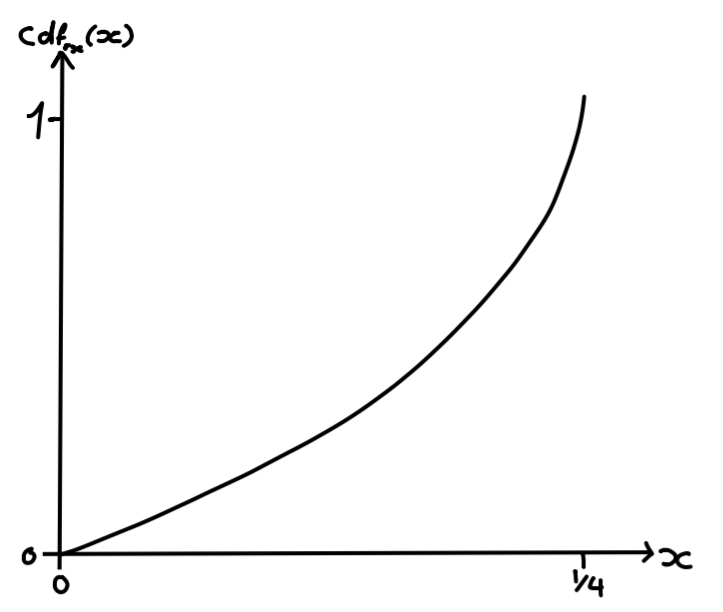
\includegraphics[width=0.5\textwidth]{./cdf_x}
\end{figure}

\[
\begin{split}
P(rx < x)
&= P(u(1 - u) < x) \\
&= P(u^2 - u + x > 0) \\
&= P\left( u < \frac{1 - \sqrt{1 - 4x}}{2} \right) + P\left( u > \frac{1 +
\sqrt{1 - 4x}}{2} \right) \\
&= \frac{1 - \sqrt{1 - 4x}}{2} + 1 - \frac{1 + \sqrt{1 - 4x}}{2} \\
&= 1 - \sqrt{1 - 4x} \\
\end{split}
\]

This is the cumulative distribution function. We can obtain the density
function by differentating this:
\[
\begin{split}
pdf_{rx}(x)
&= \pdv{x}(1 - \sqrt{1 - 4x}) \\
&= \frac{2}{\sqrt{1 - 4x}} \\
\end{split}
\]

\item We are given a dataset $x_1, \dots, x_n$ which we believe is drawn
from a $\mathcal{N}(\mu, \sigma^2)$ where $\mu$ and $\sigma$ are unknown.

\begin{enumerate}

\item Find the maximum likelihood estimators for $\hat{\mu}$ and
$\hat{\sigma}$.

\iffalse

\[
\begin{split}
\Pr(x_1, \dots, x_n \ | \ \mu, \sigma)
&= \prod^n_{i=1} \frac{1}{\sqrt{2\pi}\sigma} e^{-\frac{(\mu - x_i)
^2}{2\sigma^2}} \\
&= \frac{1}{\left(\sqrt{2\pi}\sigma\right)^n}
e^{-\frac{\sum^n_{i=1}(\mu - x_i)^2}{2\sigma^2}} \\
\ln \Pr(x_1, \dots, x_n \ | \ \mu, \sigma)
&= -\frac{n}{2}\ln(2\pi) - n\ln \sigma -\frac{\sum^n_{i=1}(\mu - x_i)^2}{2\sigma^2} \\
\end{split}
\]

We can then differentiate with respect to each variable and find the
stationary point to find the maximum likelihood estimator:

\begin{align*}
\pdv{\ln \Pr}{\mu}
&= -\frac{\sum^n_{i=1}(\mu - x_i)}{\sigma^2}
&
\pdv{\ln\Pr}{\sigma}
&= -\frac{n}{\sigma} + \frac{\sum^n_{i=1}(\mu - x_i)^2}{\sigma^3}
\end{align*}

We can now set these equal to zero and solve to find the maximum likelihood
estimators:

\[
\begin{split}
0 &= -\frac{\sum^n_{i=1}(\hat{\mu} - x_i)}{\sigma^2} \\
0 &= \sum^n_{i=1}(\mu - x_i) \\
n\mu &= \sum^n_{i=1}x_i \\
\mu &= \frac{\sum^n_{i=1}x_i}{n} \\
\end{split}
\]

Now substitute this into the equation for $\sigma$:

\[
\begin{split}
0 &= -\frac{n}{\hat{\sigma}} + \frac{\sum^n_{i=1}(\hat{\mu} - x_i)^2}
{\hat{\sigma}^3} \\
n\hat{\sigma}^2 &= \sum^n_{i=1}(\hat{\mu} - x_i)^2 \\
\hat{\sigma} &= \sqrt{\frac{\sum^n_{i=1}\left(\frac{\sum^n_{i=1}x_i]}{n} -
x_i\right)^2}{n}} \\
\end{split}
\]

\fi

\begin{lstlisting}[language=Python]
x = [...]
sigma = np.std(x)
mu = np.mean(x)
\end{lstlisting}

\item Find a 95\% confidence interval for $\hat{\sigma}$ using parametric
resampling.

\begin{lstlisting}[language=Python]
x = [...]
n = ...
stds = np.std(stats.norm.rvs(np.mean(x), np.std(x), size=(n, len(x))), axis=1)
np.quantile(stds, [0.025, 0.975])
\end{lstlisting}

\item Repeat, but using non-parametric resampling.

\begin{lstlisting}[language=Python]
x = [...]
n = ...
stds = np.std(np.random.choice(x, size=(n, len(x))), axis=1)
np.quantile(stds, [0.025, 0.975])
\end{lstlisting}

\end{enumerate}

\item The number of unsolved murders in Kembleford over three successive
years was 3, 1, 5. The police chief was then replaced and the numbers over
the following two years were 2, 3. We know from general policing knowledge
that the number of unsolved murders in a given year follows the Poisson
distribution. Model the numbers as Poisson($\mu$) under the old chief and
Poisson($\nu$) under the new chief.

\begin{enumerate}

\item Report a 95\% confidence interval for $\hat{\nu} - \hat{\mu}$ using
parametric sampling.

The maximum likelihood estimator for the parameter for a Poisson distribution
is the mean of the distribution.

\begin{lstlisting}[language=Python]
old = [3, 1, 5]
new = [2, 3]
n = ...
mu_hat = np.mean(old)
nu_hat = np.mean(new)
mu_resamp = np.mean(stats.poisson.rvs(mu_hat, size=(n, 3)), axis=1)
nu_resamp = np.mean(stats.poisson.rvs(nu_hat, size=(n, 2)), axis=1)
difs = nu_resamp - mu_resamp
np.quantile(difs, [0.025, 0.975])
\end{lstlisting}

With $n = 10000$, the confidence interval obtained is $\hat{\nu} - \hat{\mu}
 \in [-3.\.3, 2.5]$.

\item Conduct a hypothesis test of the hypothesis $\mu = \nu$, using
parametric sampling and using the test statistic $\nu - \mu$. Explain your
choice between a one-sided and a two-sided test.

We should use a two-sided test -- if $\nu - \mu$ is very small or very large
then we will reject the null hypothesis $H_0$.

Consider the null hypothesis $H_0: \mu = \nu$. We can use this assumption to
form a 95\% confidence interval for $\hat{\nu} - \hat{\mu}$. If the observed
$\hat{\nu} - \hat{\mu}$ lies outside this interval then we can reject the null
hypothesis $H_0$.

\begin{lstlisting}[language=Python]
old = [3, 1, 5]
new = [2, 3]
n = ...
mu = np.mean(np.concatenate((old, new)))
old_resamp = stats.poisson.rvs(mu, size=(n, 3))
new_resamp = stats.poisson.rvs(mu, size=(n, 2))
statistic = np.mean(new_resamp, axis=1) - np.mean(old_resamp, axis=1)
np.quantile(statistic, [0.025, 0.975])
\end{lstlisting}

Using $n = 100000$ the 95\% confidence interval obtained for $\hat{\nu} - \hat{\mu}$ was $[-3, 3]$.

Since the observed test metric, $\hat{\nu} - \hat{\mu}$ was $-\frac{1}{6}$;
which lies in the 95\% confidence interval, we do not have sufficient
evidence to reject the null hypothesis that $\mu = \nu$.

\item Explain carefully the difference in sampling methods between parts (a)
and (b).

In part (a), we did not assume the distributions were the same. Therefore we
calculated two different means and resampled from different distributions.
While in the second case, we were creating a confidence interval for
$\hat{\nu} - \hat{\mu}$ under the assumption that both data were drawn from
the same distribution. Therefore we calculated a mean for the data together
and sampled from that.

\end{enumerate}

\item In section 2.2 we considered a climate model in which temperatures
increase linearly. The probabilistic version of the model is

\[
\mathbf{temp} \sim \alpha + \beta_1\sin(2\pi\mathbf{t}) + \beta_2\cos
(2\pi\mathbf{t}) + \gamma(\mathbf{t} - 2000) + \mathcal{N}(0, \sigma^2)
\]

Find a 95\% confidence interval for $\hat{\gamma}$, the maximum likelihood
estimator for the rate of temperature increase.

\begin{lstlisting}[language=Python]
n = ...
features = np.column_stack([
	np.ones_like(climate.t),
	np.sin(climate.t),
	np.cos(climate.t),
	climate.t
])
model = LinearRegression(fit_intercept=False).fit(features, climate.temp)
model_predict = model.predict(features)
std = np.std(model_predict - climate.temp)
gammas_resamp = np.array([
	LinearRegression(fit_intercept=False).fit(features,
		stats.norm.rvs(model_predict, std)).coef_[3]
			for _ in tqdm(range(n))
])
np.quantile(gammas_resamp, [0.025, 0.975])
\end{lstlisting}

Using the data from Cambridge, the 95\% confidence interval obtained is
$\hat{\gamma} \in [0.00857158, 0.04676771]$.

\item I have defined a function for computing the fitted temperature at an
arbitrary future timepoint

\begin{lstlisting}[language=Python, mathescape=true]
def pred(t):
	return $\hat{\alpha}$ + $\hat{\beta}_1$sin(2$\pi$t) + $\hat{\beta}_2$cos(2$\pi$t) + $\hat{\gamma}$(t - 2000)
\end{lstlisting}

Modify the code to also return a 95\% confidence interval:

\begin{lstlisting}[language=Python, mathescape=true]
def pred(t):
	return stats.norm.ppf([0.025, 0.975],
		$\hat{\alpha}$ + $\hat{\beta}_1$sin(2$\pi$t) + $\hat{\beta}_2$cos(2$\pi$t) + $\hat{\gamma}$(t - 2000), $\hat{\sigma}$)
\end{lstlisting}

\item To allow for non-linear temperature increase, example sheet 1
suggested a model with a step function,

\[
\mathbf{temp} \sim \beta_1\sin(2\pi\mathbf{t}) + \beta_2\cos(2\pi\mathbf{t})
 + \gamma_{\text{decade}} + \mathcal{N}(0, \sigma^2)
\]

Find a 95\% confidence interval for $\hat{\gamma}_{\text{2010s}} -
\hat{\gamma}_{\text{1980s}}$. Conduct a hypothesis test of whether
$\gamma_{\text{1980s}} = \gamma_{\text{2010s}}$.

\begin{lstlisting}[language=Python]
n = ...
features = np.column_stack([
	np.sin(climate.t),
	np.cos(climate.t),
	*[
		climate.t // 10 == i for i in range(195, 203)
	]
])
model = LinearRegression(fit_intercept=False).fit(features, climate.temp)
std = np.std(model.predict(features) - climate.temp)
resamp = np.array([
	LinearRegression(fit_intercept=False).fit(features,
		stats.norm.rvs(climate.temp, std)).coef_
			for _ in tqdm(range(n))
])
np.quantile(resamp[:, 9] - resamp[:, 6], [0.025, 0.975])
\end{lstlisting}

Let the null hypothesis $H_0$ be $\gamma_{\text{1980s}} =
\gamma_{\text{2010s}}$. We can perform a hypothesis test by finding a 95\%
confidence interval for the difference between $\gamma_{\text{1980s}}$ and
$\gamma_{\text{2010s}}$ given the observed data. If this interval contains 0
then we will not be able to reject $H_0$ based on the observed data.

With $n = 10000$, the 95\% confidence interval obtained using the data from
Cambridge was $[-1.86936438, 2.87835352]$. Since 0 is in this interval, we
do not have sufficient evidence to reject the null hypothesis $H_0$.

\item I toss a coin $n$ times and get the answers $x_1, \dots, x_n$. My
model is that each toss is $X_i \sim B(1, \theta)$ and I wish to test the
null hypothesis $H_0$ that $\theta \geq \frac{1}{2}$.

\begin{enumerate}

\item Find an expression for $\Pr(x_1, \dots, x_n ; \theta)$. Give your
expression as a function of $y = \sum_i x_i$.

\[
\Pr(x_1, \dots, x_n) = \begin{pmatrix}
n \\ y \\
\end{pmatrix}
\theta^y(1 - \theta)^{n - y}
\]

\item Sketch $\ln \Pr(x_1, \dots, x_n ; \theta)$ as a function of $\theta$,
for two cases: $y < \frac{n}{2}$ and $y > \frac{n}{2}$.

\begin{figure}[H]
    \centering
   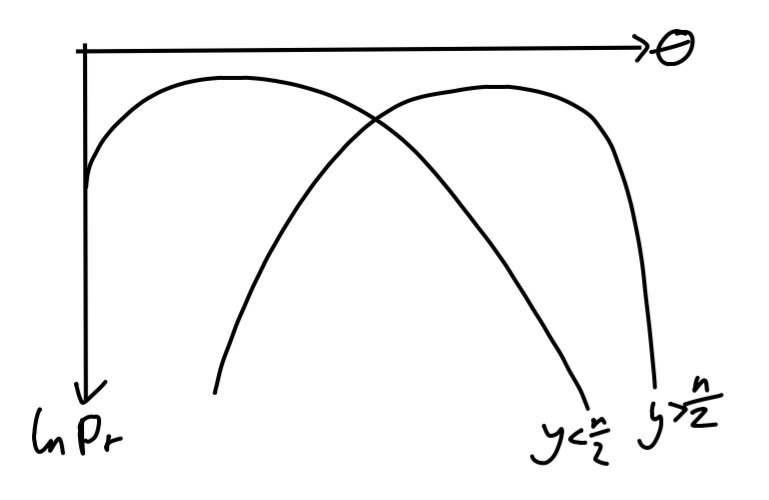
\includegraphics[width=0.7\textwidth]{./cointossing}
\end{figure}

\item Assuming $H_0$ is true, what is the maximum likelihood estimator for
$\theta$?

\[
\hat{\theta} = \max\left(\frac{y}{n}, \frac{1}{2}\right)
\]

\item Let the test statistic be $y$. What is the distribution of this test
statistic when $\theta$ is equal to your value from part (c).

\[
Y \sim B(n, \hat{\theta})
\]

\item Explain why a one-sided hypothesis test is appropriate. Give an
expression for the $p$-value of the test.

We are only interested in the probability that $\theta < \frac{1}{2}$. We
are not interested in the possibility that it is greater than $\frac{1}{2}$
and therefore should not be convinced by a very large value for $y$ --
however this is what a two-sided test would do.

\[
p = \sum^{y}_{i=0} \begin{pmatrix}
n \\ i \\
\end{pmatrix} \frac{1}{2}^i\cdot\frac{1}{2}^{n - i}
\]

\end{enumerate}

\item Your attempts at a task succeed with probability $\theta$ and fail
with probability $1 - \theta$. How long an unbroken list of failures does it
take for you to reject ``$\theta \geq \frac{1}{2}$'' at $p$-value 5\%?

Assuming the only data that we have is this list of failures, a list of
failures of length $\lceil-\log_2 0.05\rceil = 5$ would be sufficient to
convince us with 95\% confidence that the probability of success was $<
\frac{1}{2}$

\end{enumerate}

\section{Supplementary questions}

\begin{enumerate}

\setcounter{enumi}{8}

\item A point lightsource at coordinates (0, 1) sends out a ray of light at
an angle $\Theta$ chosen uniformly in $ \left( -\frac{\pi}{2}, \frac{\pi}{2}
\right) $. Let $X$ be the point where the ray intersects the horizontal line
through the origin. What is the density of $X$?

\[
\begin{split}
P(X < x)
&= P(\tan(u) < x) \\
&= P(u < \arctan(x)) \\
&= \frac{\frac{\pi}{2} + \arctan(x)}{\pi} \\
&= c \\
\end{split}
\]

We can differentiate this to find the probability density function for $x$:

\[
\begin{split}
\text{pdf}(x)
&= \pdv{x}\left(\frac{\pi + 2\arctan(x)}{2\pi}\right) \\
&= \frac{1}{\pi(1 + x^2)}
\end{split}
\]


\item We are given a dataset $x_1, \dots, x_n$ which we believe is drawn
from $\mathcal{U}[0, \theta]$ where $\theta$ is unknown. Recall from example
sheet 1 that the maximum likelihood estimator is $\hat{\theta} = \text{max}_i
x_i$. Find a 95\% confidence interval for $\hat{\theta}$, both using
parametric resampling and using non-parametric resampling.

Parametric Resampling:

\begin{lstlisting}[language=Python]
num_tests = ...
rands = np.random.random((num_tests, x.size))
max_gen = np.max(rands, axis=1)
ratio = 1 / max_gen
np.max(x) * np.quantile(ratio, [0, 0.95])
\end{lstlisting}

Non-parametric Resampling:

\begin{lstlisting}[language=Python]
largest = np.max(x)
gen_data = np.random.choice(x, size=(num_tests, x.size))
max_gen = np.max(gen_data, axis=1)
ratio = np.max(x) / max_gen
np.max(x) * np.quantile(ratio, [0, 0.95])
\end{lstlisting}

\item I implement the two resamplers from question 10. To test them, I
generate 1000 values from $\mathcal{U}[0, \theta]$ with $\theta = 2$ and
find a 95\% confidence interval for $\hat{\theta}$. I repeat this 20 times.
Not once does my confidence interval include the true value, $\theta = 2$
for either resampler. Explain.

I did not observe behaviour like this:

\begin{itemize}

\item
For the parametric resampler, I observed \~95\% of confidence intervals
containing the true maxima -- this result occurred for all 95\% confidence
intervals ie [0\%, 95\%], [2.5\%, 97.5\%], [5\%, 100\%].

\item
For the non-parametric resampler, I observed between 80\% and 90\% of
confidence intervals containing the correct value with 1000 attempts
(depending on which confidence interval I chose).

\end{itemize}

I believe the answer Damon wants is along the lines of: ``by definition this
question is asking us to extrapolate''. We are not fitting (and cannot fit)
any model which is good at extrapolating. Therefore the question is
inherently unsuited to frequentist approaches and even a well-fit model will
not perform well when we are forced to extrapolate.

\item Test the hypothesis that temperatures in Cambridge have not been
changing, using a non-parametric test.

I will assume that temperatures in each month are sampled from some
distribution. Therefore I will only shuffle the months. I will
non-parametrically resample the temperature for a given day in a month
from the set of temperatures which happened in that month.
I will then use the MLE for $\gamma$ as the readout statistic and find a
confidence interval on that.

The code is implemented below:

\begin{lstlisting}[language=Python]
gammas = []

for tests in tqdm(range(25000)):
    temp = np.copy(climate.temp)
    for i in range(12):
        temp[climate.mm == i] = np.random.choice(
        	temp[climate.mm == i], size=np.count_nonzero(climate.mm == i))
    gammas.append(LinearRegression(fit_intercept=False).fit(features, temp).coef_[3])
\end{lstlisting}

The 95\% confidence interval fora  two tailed test is
$[-0.000549, 0.010008]$. The observed $\hat{\gamma}$ is 0.029218927735124786
-- which is outside the range. Therefore, we can conclude with 95\%
confidence that the temperature in Cambridge is changing.

\item We have a dataset $x_1, x_2, \dots, x_n$ and we wish to model it as
$\mathcal{N}(\mu, \sigma^2)$ where $\mu$ and $\sigma$ are unknown. How
different are Bayesian and frequentist confidence intervals for the mean? To
be concrete, lets work with the first 10 values for \texttt{temp} in the
climate dataset.

\begin{enumerate}

\item Plot the log likelihood function $\ln\Pr(x_1, \dots, x_n | \mu,
\sigma)$ as a function of $\mu$ and $\sigma$.

\begin{lstlisting}[language=Python]

\end{lstlisting}

\begin{figure}[H]
\centering
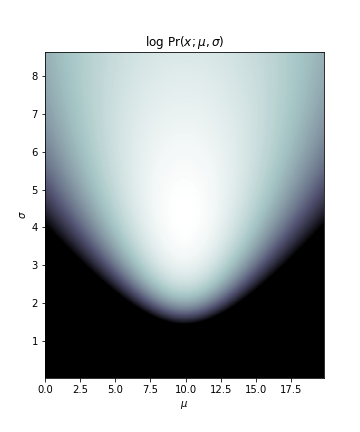
\includegraphics[width=0.5\textwidth]{./q13_a_logPr}
\end{figure}

\item Using frequentist resampling, generate 50 resampled datasets, find
the maximum likelihood estimators $\hat{\mu}$ and $\hat{\sigma}$ for each
and show these 50 points on your plot.

\begin{figure}[H]
\centering
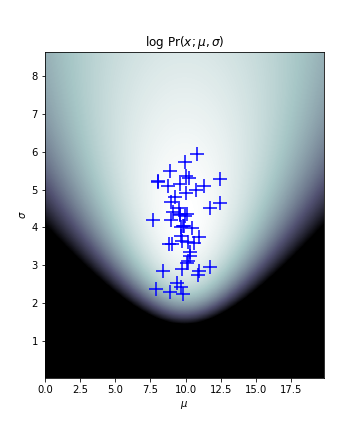
\includegraphics[width=0.5\textwidth]{./q13_b_frequentist}
\end{figure}

\item Using computational Bayesian methods, with priors $\mu \sim
\mathcal{N}(0, 10^2)$ and $\sigma \sim \Gamma(k=2, \theta =1)$ (where $k$)
and $\theta$ are as in the numpy documentation), sample 500 pairs from the
prior distribution and show them on your plot. Then compute the posterior
weights of these sampled pairs and show the weigthed pairs on your plot by
setting the size of the plot marker in proportion to weight.

\begin{figure}[H]
\centering
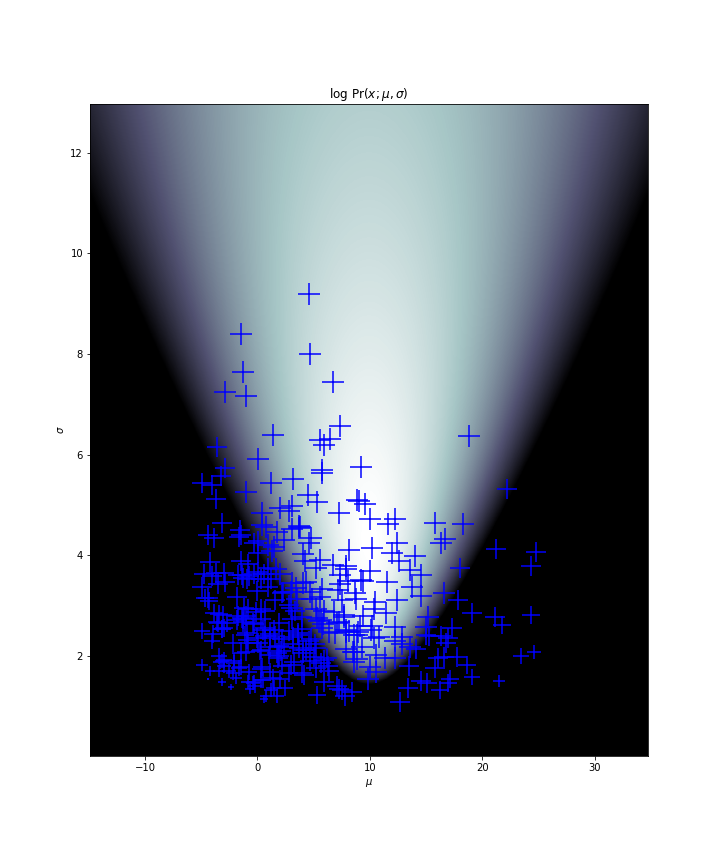
\includegraphics[width=0.5\textwidth]{./q13_c_bayesian}
\end{figure}


\item Find the 95\% confidence interval (for $\hat{\mu}$ in the frequentist
case and for $(\mu | \text{data})$ in the Bayesianist case) and show them on
your plot.

\begin{figure}[H]
\centering
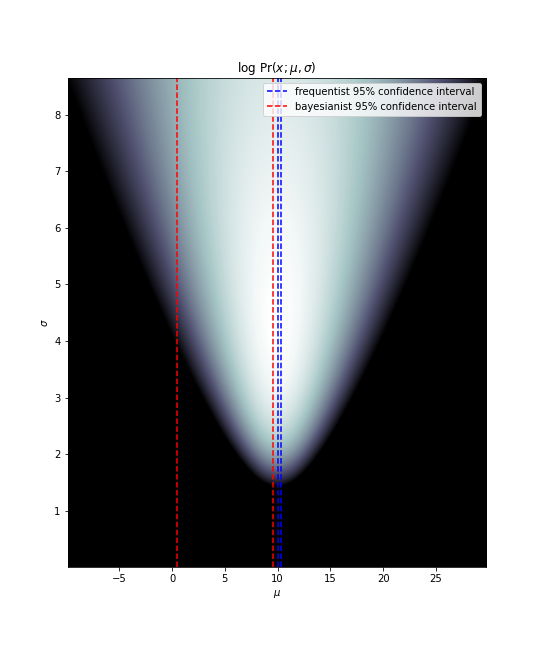
\includegraphics[width=0.5\textwidth]{./q_13_d_frequentist_bayesian}
\end{figure}


\item Repeat the exercise, using the first 100 values from the climate dataset.

A plot of the log likelihood function of the first 100 data values versus
$\mu$, $\sigma$:

\begin{figure}[H]
\centering
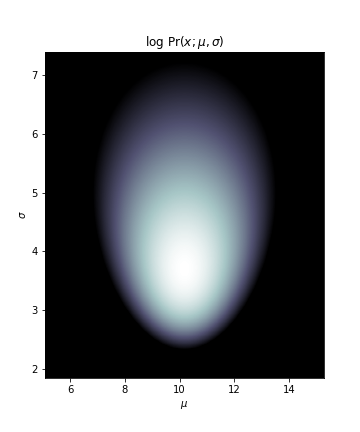
\includegraphics[width=0.5\textwidth]{./q13_a_logPr_100}
\end{figure}

A scatter diagram of the observed means and stanard deviations of
parametrically resampled datasets:

\begin{figure}[H]
\centering
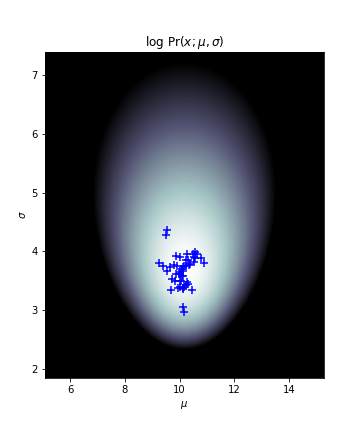
\includegraphics[width=0.5\textwidth]{./q13_b_frequentist_100}
\end{figure}

A scatter diagram of the bayesian samples with cross size scaled by log
probability:

\begin{figure}[H]
\centering
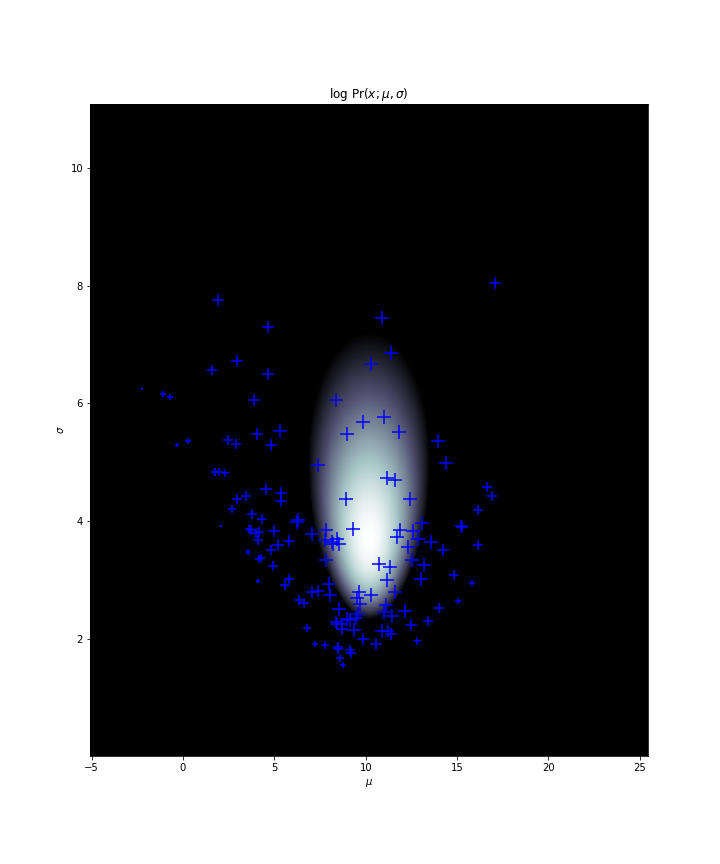
\includegraphics[width=0.5\textwidth]{./q13_c_bayesian_100}
\end{figure}

Bayesian and frequentist confidence intervals:

\begin{figure}[H]
\centering
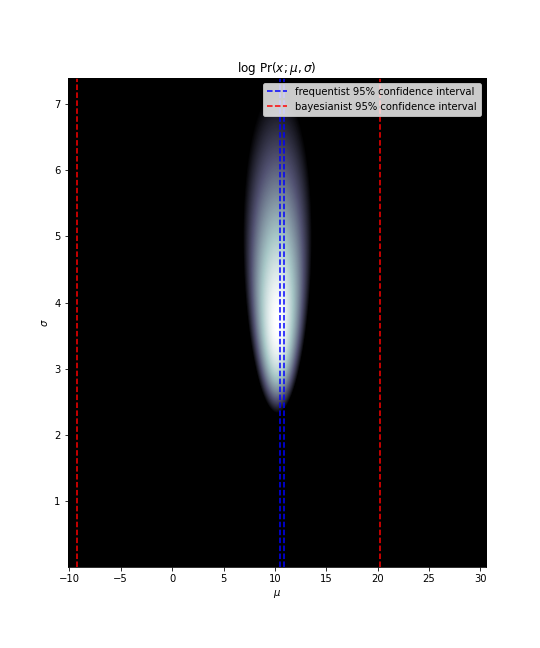
\includegraphics[width=0.5\textwidth]{./q_13_d_frequentist_bayesian_100}
\end{figure}

\end{enumerate}

\item In hypothesis testing, what $p$-value would you expect if $H_0$ is true?

If $H_0$ is true, I would expect $p \sim \mathcal{U}[0, 1]$.

\iffalse

\item We are given a dataset $x_1, \dots, x_n$. Our null hypothesis is that
these values are drawn from $\mathcal{N}(0, \sigma^2)$ where $\sigma$ is an
unknown parameter. Let

\[
\hat{F}(x) = \frac{1}{n}\sum^{n}_{i=1} 1[x_i/\hat{\sigma}\leq x]
\]

where $\hat{\sigma} = \sqrt{\frac{\sum^n_{i=1}x_i^2}{n}}$ is the maximum
likelihood estimator for $\sigma$. If the null hypothesis is true, we'd
expect $\hat{F}(x)$ to be reasonably close to $\Phi(x)$, the cumulative
distribution function for $\mathcal{N}(0, 1)$ for all $x$. Suggest how to
test the hypothesis that the dataset is indeed drawn from $\mathcal{N}(0,
\sigma^2)$ using a test statistic based on $\hat{F}$ and $\Phi$.

The easiest test statistic is to use parametric resampling to find a 95\%
confidence interval for $\hat{F}(1) - \hat{F}(-1)$ for data of size $n$.

\begin{lstlisting}[language=Python]
tests = ...
resampled = stats.norm.rvs(0, 1, size=(tests, n))
f1 = np.count_nonzero(resampled < 1, axis=1)
fminus1 = np.count_nonzero(resampled < -1, axis=1)
np.quantile(f1 - fminus1, [0.025, 0.975])
\end{lstlisting}

If the value for $\hat{F}(1) - \hat{F}(-1)$ is outside the quantiles
generated, then we will have sufficient evidence to reject the null
hypothesis that $X\sim\mathcal{N}(0, \sigma)$.

\item

\begin{enumerate}[label=(\alph*)]

\item Let $T$ be the maximum of $m$ independent $\mathcal{U}[0, 1]$ random
variables. Show that $\mathbb{P}(T \leq t) = t^m$. Find the density function
$\text{Pr}_T(t)$

\[
\begin{split}
P(T \leq t)
&= P(x_0 \leq t) \cdot \dots P(x_n \leq t) \\
&= t \cdot \dots \cdot t \\
&= t^n \\
\end{split}
\]


\item A common task in data processing is counting the number of unique
items in a collection. When the collection is too large to hold in memory,
we may wish to use fast approximation methods such as the following: Given a
collection of items $a_1, a_2, \dots$ compute the hash of each item
$x_1 = h(a_1)$, $x_2 = h(a_2)$, \ldots then compute $t = \text{max}_i x_i$.

If the hash function is well designed, then each $x_i$ can be treated as if
it were sampled from $\mathcal{U}[0, 1]$ and unequal items will yield
independent samples.

The more unique items there are, the larger we expect $t$ to be. Given an
observed value $t$, find the maximum likelihood estimator for the number of
unique items.

\[
P(T \leq t)
= t^n
\]

For all $n \in \mathbb{Z}$. $t^{n + 1} < t^n$. Therefore the maximum
likelihood estimator is $n = 1$.

\end{enumerate}

\item A recent paper \textit{Historical language records reveal a surge of
cognitive distortions in recent decades} claims that depression-linked turns
of phrase have become more prevent in recent decades. this paper reports
both confidence intervals and null hypotheses. Explain how it computes them,
in particular (1) the readout statistic and (2) the sampling method.

The readout statistic is the z-score for frequency of n-grams relating to
depression as a proportion of all n-grams in literature that year estimated
by the number of end-of-sentence markers.

The null hypothesis is that the depression-related n-grams are changing no
more than any other n-grams. The confidence intervals for the null hypothesis
was calculated by selecting the same number of the same length of n-grams as
the depression-related n-grams and creating confidence intervals on their
z-scores. It is observed that the null hypothesis is broadly uncorrelated with
the observed frequency for depression-related n-grams.

\fi

\end{enumerate}

\begin{examquestion}{2020}{6}{8}

This table shows a summary of temperature readings from the Cambridge
weather station, comparing June, July and August in the 1970s to the 2010s.
It shows the number of months in which the average maximum daily temperature
was low (< 15.5$^\circ$C), high (> 18$^\circ$C) or medium. We wish to
establish whether there is a significant difference between the two rows.

\begin{table}[H]
\centering
\begin{tabular}{l l l l}
& low & med & high \\
\hline
1970s & 10 & 18 & 2 \\
2010s & 5 & 14 & 11 \\
\end{tabular}
\end{table}

Suppose that readings are independent from month to month. let $p_{d, k}$ be
the probability that a month's reading falls into bin $k \in \{\text{low},
\text{med}, \text{high}\}$ in decade $d \in \{1970s, 2010s\}$. The $p_{d,
k}$ are unknown parameters.

\begin{enumerate}[label=(\alph*)]

\item Give expressions for the maximum likelihood estimates $\hat{p}_{d, k}$.
In your answer, you should state what is being maximised over what variables.

\[
\hat{p}_{d,k} = \frac{n_{d,k}}{n_{d}}
\]

Where:

\begin{itemize}

\item $p_{d,k}$ is the probability of the months reading falling into the
bin $k$.

\item $n_{d,k}$ is the number of months in decade $d$ which fell into bin $k$.

\item $n_d$ is the number of months in decade $d$.

\end{itemize}

\item Let the null hypothesis $H_0$ be that the probabilities are the same
in the 1970s as in teh 2010s; call these common probabilities $q_k$. Give
expressions for the maximum likelihood estimates $\hat{q}_k$ under $H_0$.

\[
\hat{q}_k = \frac{n_k}{n}
\]

Where:

\begin{itemize}

\item $n_k$ is the number of months in the 1970s and 2010s where the reading
fell into bin $k$.

\item $n$ is the number of months in the 1970s and 2010s.

\end{itemize}

\item We wish to test $H_0$ using the test statistic

\[
t = \sum_{d,k}  \frac{\left( \hat{p}_{d,k} - \hat{q}_k \right)^2}{\hat{q}_k}
\]

\begin{enumerate}[label=(\roman*)]

\item Explain briefly what is meant by \textit{parametric resampling}.
Explain how to compute the distribution we'd expect to see for $t$ under
$H_0$. Give pseudocode.

Parametric resampling is the process of approximating the distribution for a
readout statistic by fitting a model to the data and then resampling the
data from this model and generating the readout statistic for each of those
data. We can then visualise this distribution of statistics either by
creating confidence intervals or by making a histogram.

\begin{lstlisting}[language=Python, mathescape=true]
$\hat{\theta}$ = calculate_statistic(data)
resampled = fitted_model.rvs(size=(n, *data.shape))
statistic = calculate_statistic_vectorised(resampled)
low, high = quantile(statistic, [$p_{lo}$, $p_{hi}$])
plt.hist(statistic)
\end{lstlisting}

\item Explain what is meant by a one-sided test versus a two-sided test.
Which should we use in this case?

A two-sided test can be used to test if a statistic is \textit{different} to
a particular value; while one-sided tests are used to test whether a
statistic is greater than a value; or a different one-sided test can be used
to test whether a statistic is less than a value.

We should use a two-sided test when we wish to test for significant evidence
that a statistic is \textit{not equal to} a certain value. We use a
one-sided test to test when we have a belief about whether the statistic is
greater than or less than that value -- for example testing if a probability
is $> \frac{1}{2}$.

\item Give pseudocode to compute the $p$-value of this test.

In this case, we are testing the assumption $H_0$ and therefore we should
perform a two-sided hypothesis test.

\begin{lstlisting}[language=Python, mathescape=true]
# calculate maximum likelihood estimators from observed data
$\hat{p}$, $\hat{q}$ = calculate_mles(data)
# generate $n$ new resampled data
resampled = np.choice(['lo','med','hi'], p=$\hat{q}$, size=(n, *data.shape))
# calculate the statistic we are interested in for each
# of these resampled distributions
resampled_t = [t(calculate_mles(resampled_i)) for resampled_i in resampled]
# work out a two-sided 95% confidence interval
lo, hi = np.quantile(resampled_t, [0.025, 0.975])
# if false we can reject $H_0$
lo < t($\hat{p}$, $hat{q}$) < hi
\end{lstlisting}

\end{enumerate}

\item What are some advantages and disadvantages of this count-based test,
compared to a test based on linear regression?

Advantages:

\begin{itemize}

\item Results are easier to interpret

\item Making good statistics is easier than a linear regression based test

\item Can be less computationally expensive

\end{itemize}

Disadvantages:

\begin{itemize}

\item Does not fully use data

\item Counts may be adversarially chosen, leading to invalid conclusions

\item Ignores extreme values

\end{itemize}

\end{enumerate}

\end{examquestion}

\end{document}
